\chapter{天体物理学}\label{ch:b3:astrophysics}

% Provenance (not for print): the astrophysics option offered across the
% surveyed third-year curricula, built here as a capstone that reuses the
% whole volume (Fermi gas -> white dwarfs, nuclear -> stellar burning,
% Planck law -> CMB, Saha -> recombination).

本书每一章都在为本章做准备。恒星
是由本科一年级分册的流体静力学支配的自引力气体球，
由\cref{ch:b3:nuclear-physics}中的隧道效应点燃，
依\cref{ch:b3:photons-phonons}中的普朗克定律发光；死亡的恒星是
\cref{ch:b3:quantum-statistics}中的简并费米气体，大小如
城市；而宇宙本身是一个正在冷却的热力学系统，其
“婴儿照”——宇宙微波背景——是迄今测得的最完美的
黑体。本章作为收尾，把全书汇集成
一座尽可能大的实验室：恒星如何“生”，
如何“死”，留下什么，以及包含它们的膨胀宇宙
如何起源于我们已完成的物理。

\section{恒星是一种平衡}

\begin{proposition}[流体静力平衡]\label{prop:b3:astrophysics:hydrostatic}
\index{恒星流体静力平衡}\index{恒星结构}
恒星既不坍缩也不散开：在每一半径处，
压强梯度承载着上方气体的重量。记
$m(r)$ 为半径 $r$ 以内的质量，
\[
\frac{\dd P}{\dd r} = -\frac{Gm(r)\rho(r)}{r^2} .
\]
对整个太阳估算，$P_{\text{c}} \sim GM^2/R^4 \sim
\qty{e15}{Pa}$，由理想气体状态方程可得 $T_{\text{c}} \sim
10^7\,\unit{K}$（见\cref{exo:b3:astrophysics:1}）——恰好是
\cref{exo:b3:nuclear-physics:11}中的质子
开始隧穿的温度。这并非巧合，而是热源式的自调节：恒星
\emph{必须}收缩并升温，直到核心点燃，而聚变
此后维持平衡，持续数百万至数十亿年。恒星
具有负热容——失去能量、收缩、反而
变得\emph{更热}（见\cref{exo:b3:astrophysics:5}）——这正是
引力终将胜出的原因。
\end{proposition}

\begin{proof}
位于 $[r, r + \dd r]$ 的薄壳层，面积为 $A$，下方受压力 $P(r)A$，
上方受压力 $P(r + \dd r)A$，并受重力 $g\rho A\,\dd r$，
其中 $g = Gm(r)/r^2$（仅内部质量产生吸引，据引力的高斯
定理）。三力平衡给出所述的
方程。
\end{proof}

\begin{omfigure}
\begin{tikzpicture}[scale=1.0]
  \fill[omExo!14] (0,0) circle (2.2);
  \fill[omExo!30] (0,0) circle (1.15);
  \draw[omDef, thick] (0,0) circle (2.2);
  \draw[omDef!60] (0,0) circle (1.15);
  \node[font=\scriptsize, align=center] at (0,0)
    {核心 \\$10^7\,\unit{K}$：聚变};
  % pressure arrows outward
  \foreach \ang in {25,115,205,295}
    \draw[->, omThm, thick] (\ang:1.25) -- (\ang:1.8);
  \node[omThm, font=\scriptsize, anchor=west] at (2.5,0.85)
    {压力向外推};
  % gravity arrows inward
  \foreach \ang in {70,160,250,340}
    \draw[->, omDef, thick] (\ang:2.75) -- (\ang:2.3);
  \node[omDef, font=\scriptsize, anchor=west] at (2.5,-0.85)
    {引力向内拉};
\end{tikzpicture}

{\small 将恒星本身画成受力图。聚变驱动
承托恒星自身重力的压强；两种力
相互博弈了一百亿年——本章中的每一种恒星归宿，
都是其中一方“理屈词穷”时的结局。}
\end{omfigure}

\section{恒星的一生}

\begin{definition}[赫茨普龙–罗素图]\label{def:b3:astrophysics:hr}
\index{赫茨普龙–罗素图}\index{主序}
以表面温度（按惯例，热者在\emph{左侧}）
对亮度作图，二者均取自
\cref{ch:b3:photons-phonons}中的黑体定律，它们
并不散乱：约百分之九十挤在\emph{主序}上，
即由氢燃烧星构成的斜向带，其排列完全由质量决定——
质量越大则温度越高，\emph{且}亮度远超比例增长
（$L \propto M^{3.5}$），因而寿命更短
（$t \propto M/L \propto M^{-2.5}$：
见\cref{exo:b3:astrophysics:4}）。带外居住着
图中的例外与归宿：温度低而体积庞大的\emph{巨星}
（位于右上），以及温度高而体积极小的\emph{白矮星}（位于左下）
——因为在温度固定时，由 $L = 4\pi R^2\sigma T^4$，
亮度是\emph{大小}的度量。赫茨普龙–罗素图并非
一张划分种类的图，而是标示\emph{年龄}的图：恒星的点
在图上漂移，随燃料耗尽而移动。
\end{definition}

\begin{omfigure}
\begin{tikzpicture}
  \begin{axis}[omaxis, axis x line=bottom, axis y line=left,
    width=9.8cm, height=6.8cm, xmin=0, xmax=10, ymin=-4.6, ymax=6.4,
    xlabel={表面温度（热 $\to$ 冷）},
    ylabel={$\log_{10}(L/L_\odot)$},
    xlabel style={at={(axis description cs:0.5,-0.08)}, anchor=north},
    xtick=\empty, ytick={-4,-2,0,2,4,6}, clip=false]
    % main sequence band
    \addplot[omDef, line width=5pt, opacity=0.28, domain=0.6:9.4]
      {5.0 - 1.05*x};
    \addplot[omDef, thick, domain=0.6:9.4] {5.0 - 1.05*x};
    % sun
    \fill[omExo] (axis cs:4.76,0) circle (2pt);
    \node[omExo, font=\scriptsize, anchor=north east] at (axis cs:4.6,-0.4)
      {太阳};
    % giants
    \fill[omThm!25] (axis cs:8.1,3.4) ellipse (1.35 and 1.0);
    \node[omThm, font=\scriptsize] at (axis cs:8.1,3.4) {巨星};
    % white dwarfs
    \fill[gray!25] (axis cs:2.6,-3.2) ellipse (1.5 and 0.75);
    \node[font=\scriptsize] at (axis cs:2.6,-3.2) {白矮星};
    \node[omDef, font=\scriptsize, rotate=-38, anchor=south] at
      (axis cs:2.6,2.5) {主序};
  \end{axis}
\end{tikzpicture}

{\small 赫茨普龙–罗素图。主序是
氢燃烧的带状区域，是一道质量阶梯：从左上角
蓝色、挥霍无度、数百万年便寿终的恒星，到右下角的
红色、节俭、寿命至今仍超过宇宙年龄的恒星。巨星与白矮星
并非异常，而是章节：同一颗恒星会依次经历这三个区域。}
\end{omfigure}

\begin{remark}[恒星如何老化，以及留下什么]\label{rem:b3:astrophysics:evolution}
\index{红巨星}\index{超新星}\index{核合成（恒星）}
核心的氢耗尽后，热源式的调节逻辑重新上演：
核心收缩升温，氦被点燃（聚变为碳
和氧），外层膨胀百倍 --- 成为红巨星。
类太阳恒星止步于此：它抛掉外层，
退役成为白矮星。质量高于 $\approx8M_\odot$ 的恒星则不断点燃
洋葱状壳层中的新燃料，直到核心成为\emph{铁} ---
\cref{prop:b3:nuclear-physics:binding}中的峰顶，此后
聚变不再释放能量。垂死的核心在一秒之内坍缩；
反弹与中微子洪流将恒星炸开，形成一次
\emph{超新星}，短暂地盖过所在星系的光芒，并以中子俘获锻造出
比铁更重的元素，并把这些物质
抛入孕育下一代恒星与行星的星云中。你骨骼里的钙和
血液里的铁，都走过这条路径（\cref{pb:b3:astrophysics:1}）：
化学不过是
循环利用的天体物理学。
\end{remark}

\section{遗骸：处于极限的物质}

\begin{proposition}[白矮星与中子星]\label{prop:b3:astrophysics:compact}
\index{白矮星}\index{中子星}\index{钱德拉塞卡质量}\index{黑洞}\index{史瓦西半径}
是什么托住一颗不再燃烧的恒星？答案是量子力学。一颗
\emph{白矮星}是约一个太阳质量的碳与氧，靠其
\emph{电子简并压}撑住 --- 即 $T = 0$ 时的费米压（见
\cref{ch:b3:quantum-statistics}） --- 体积与地球相当，
每茶匙重一吨。泡利的支撑有上限：超过
\emph{钱德拉塞卡质量} $M_{\text{Ch}}
\approx 1.4\,M_\odot$ 时，电子变为相对论性，
压强输掉这场竞争（在本阶段不加证明地承认）。超过此值后，
电子被挤压进质子，形成\emph{中子星}：中子简并与核斥力
共同托住
$\sim1.4\,M_\odot$ 的质量，压缩在约十二千米之内，达到
\cref{def:b3:nuclear-physics:nuclide}中的核密度 --- 一个
城市大小的原子核，自转可快至毫秒量级，并像灯塔一样扫射（即
\emph{脉冲星}）。而超过约 $3\,M_\odot$ 时，
已知没有东西能抵抗：恒星会落入某一半径之内，
在该半径处逃逸需要光速，
\[
R_{\text{s}} = \frac{2GM}{c^2}
\qquad (\qty{3}{km}\text{ 每太阳质量}) ,
\]
即\emph{黑洞} --- 引力的最后定论，并且是广义相对论的
门槛，留待本套书的下一分册。
\end{proposition}
\admitted

\begin{omfigure}
\begin{tikzpicture}[scale=1.0]
  % log-scale size ladder
  \draw[omDef, fill=omExo!18, thick] (0,0) circle (1.9);
  \node[font=\scriptsize, align=center] at (0,-2.35)
    {太阳 \\$7\times10^5$ km};
  \draw[omDef, fill=omDef!15, thick] (4.4,0) circle (0.55);
  \node[font=\scriptsize, align=center] at (4.4,-2.35)
    {白矮星 \\$\sim\qty{7000}{km}$};
  \draw[omThm, fill=omThm!18, thick] (7.3,0) circle (0.16);
  \node[font=\scriptsize, align=center] at (7.3,-2.35)
    {中子星 \\$\sim\qty{12}{km}$};
  \fill (9.7,0) circle (0.06);
  \node[font=\scriptsize, align=center] at (9.7,-2.35)
    {黑洞 \\$R_{\text{s}} \sim \qty{4}{km}$};
  \node[font=\scriptsize, gray, anchor=south, align=center] at (4.85,1.55)
    {质量相近，引力愈来愈强 \\（尺寸未按比例）};
\end{tikzpicture}

{\small 同为一个太阳质量，四种尺度。热压强支撑着
太阳；电子简并支撑白矮星；中子简并支撑
中子星；无物支撑黑洞。每一步使
表面引力增大约一万倍 --- 以及站稳脚跟所需的
物理也随之增多。}
\end{omfigure}

\section{膨胀的宇宙}

\begin{definition}[哈勃定律与炽热的开端]\label{def:b3:astrophysics:hubble}
\index{哈勃定律}\index{宇宙微波背景}\index{大爆炸核合成}
每个遥远的星系都在退行，其退行速率与距离成正比：
\[
v = H_0d , \qquad H_0 \approx \qty{70}{km/s}
\text{ 每兆秒差距} .
\]
这不是\emph{进入}空间的爆炸，而是
\emph{空间}本身的膨胀 --- 倒推回去，一切曾经
致密而炽热：$1/H_0 \approx 14$ 十亿年前
（见\cref{exo:b3:astrophysics:9}）。早期宇宙就是
加速重放的本书。一秒时，它是一锅 \unit{MeV} 粒子浓汤
（见\cref{ch:b3:particle-physics}）；最初几分钟里，
在\cref{ch:b3:nuclear-physics}中，核反应剧烈进行，并
\emph{按质量计四分之一为氦} --- 由玻尔兹曼
因子预言，并处处被观测到。
（见\cref{exo:b3:astrophysics:11}）。在 380\,000 年、
\qty{3000}{K} 时，萨哈方程
（见\cref{prop:b3:grand-canonical:saha}）使电子终于
与质子结合；迷雾散去，那束最后一次散射的光 ---
因膨胀而拉伸了千倍 --- 今天以
\emph{宇宙微波背景}：一条 \qty{2.725}{K} 的普朗克谱
（见\cref{ch:b3:photons-phonons}），是现存最古老的
照片。这幅图还显示，星系的自转与聚集
仿佛受一种任何探测器都未曾捕获的\emph{暗物质}操控，而且
膨胀\emph{正在加速}，受一种\emph{暗能量}驱动，
至今无人解释 --- 即占宇宙预算的百分之九十五，
本书目前尚无法写清。
\end{definition}

\begin{omfigure}
\begin{tikzpicture}
  \begin{axis}[omaxis, axis x line=bottom, axis y line=left,
    width=9.6cm, height=5.8cm, xmin=0, xmax=105, ymin=0, ymax=8.4,
    xlabel={距离 (\unit{Mpc})},
    ylabel={退行速率 ($10^3\,\unit{km/s}$)},
    xlabel style={at={(axis description cs:0.5,-0.1)}, anchor=north},
    xtick={25,50,75,100}, ytick={2,4,6,8}, clip=true]
    \addplot[omDef, thick, domain=0:103] {0.07*x};
    \addplot[only marks, mark=*, mark size=1.4pt, omThm]
      coordinates {(9,0.75) (17,1.05) (24,1.85) (31,2.0) (39,2.9)
        (46,3.05) (54,3.95) (61,4.1) (69,5.05) (76,5.15)
        (84,6.05) (91,6.2) (98,7.0)};
    \node[omDef, font=\scriptsize, anchor=north west] at (axis cs:57,3.6)
      {斜率 $H_0$};
  \end{axis}
\end{tikzpicture}

{\small 哈勃定律：退行速率随距离的变化，每个点
代表一个星系（速率由多普勒频移得到，
见\cref{ch:b3:relativistic-kinematics}；距离由标准
烛光得到）。斜率为 $H_0$；其倒数大致为
宇宙的年龄。}
\end{omfigure}

\begin{omfigure}
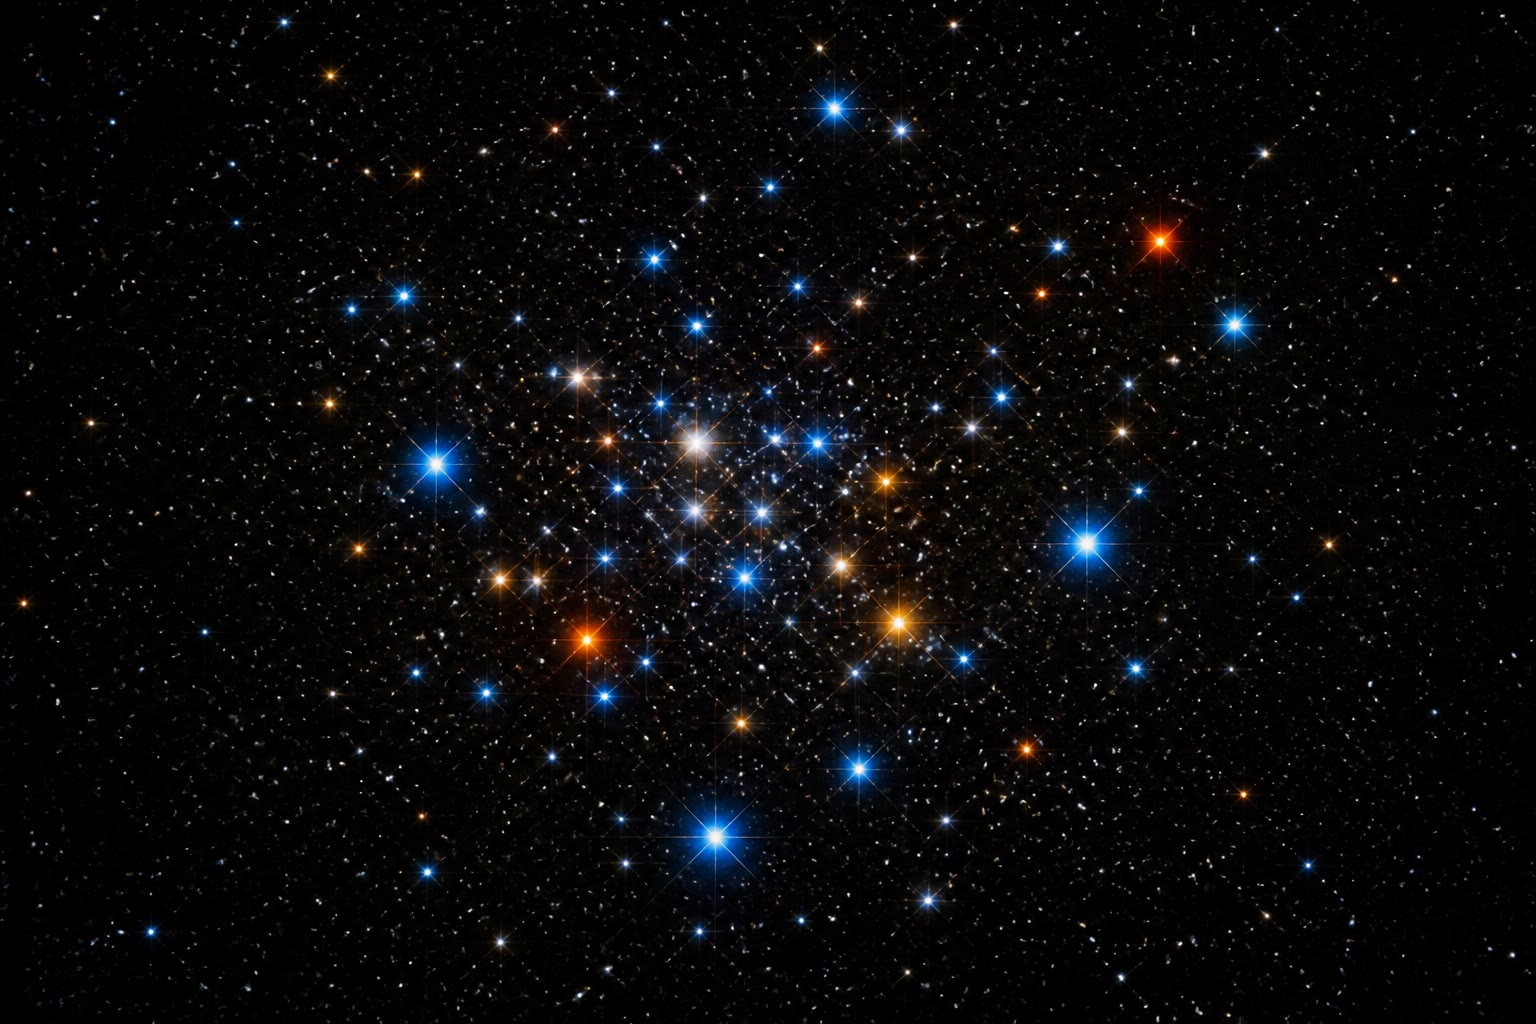
\includegraphics[width=0.58\linewidth]{images/book5/ai/b5-23-star-colors.jpg}

{\small 一个疏散星团：蓝白色的“挥霍者”与节俭的橙色矮星同时诞生，却以截然不同的速率老化 --- 赫茨普龙–罗素图的实拍照片。}
\end{omfigure}

\section{练习}

\begin{exercise}[$\star$]\label{exo:b3:astrophysics:1}
太阳的估算：$M = \qty{2e30}{kg}$，$R = \qty{7e8}{m}$。
(a) 估算 $P_{\text{c}} \sim GM^2/R^4$。(b) 利用平均
密度与理想气体定律（$P = \rho k_{\text{B}}T/
m_{\text{p}}$），估算 $T_{\text{c}}$。(c) 将其与
$10^7\,\unit{K}$ 的点火阈值相比较（见
\cref{exo:b3:nuclear-physics:11}）。(d) 为何这一吻合
是热源式的调节，而非巧合？
\end{exercise}

\begin{exercise}[$\star$]\label{exo:b3:astrophysics:2}
光度测定。(a) 由太阳常数
\qty{1360}{W/m^2}（距离 $d = \qty{1.5e11}{m}$ 处），求
$L_\odot$。(b) 由 $L = 4\pi R^2\sigma T^4$ 求
太阳表面温度。(c) 检验维恩峰值与太阳的
可见黄绿光是否相符。(d) 每一步分别用到了哪一章的定律？
\end{exercise}

\begin{exercise}[$\star$]\label{exo:b3:astrophysics:3}
读图。天狼星 B：$T \approx \qty{25000}{K}$，$L
\approx 0.026\,L_\odot$；参宿四：$T \approx \qty{3500}{K}$，
$L \approx 10^5\,L_\odot$。(a) 将两者标在赫茨普龙–罗素图上。(b)
由 $L = 4\pi R^2\sigma T^4$ 求两者的
以太阳为单位的半径。(c) 若将参宿四置于太阳系中，哪些行星
会位于其内？(d) 是什么支撑着天狼星 B 不致坍缩？
\end{exercise}

\begin{exercise}[$\star$]\label{exo:b3:astrophysics:4}
活得快，死得早。已知 $L \propto M^{3.5}$ 及寿命
$t \propto M/L$，太阳寿命为一百亿年：(a) 求
质量为 $10\,M_\odot$ 的恒星的寿命；(b) 求质量为 $0.5\,M_\odot$ 的红矮星的寿命 ---
与宇宙年龄比较；(c) 为何质量更大的恒星拥有
\emph{更多}燃料，却\emph{更早}死亡？(d) 大质量恒星寿命如此短暂，
说明超新星发生在
星系的何处？
\end{exercise}

\begin{exercise}[$\star\star$]\label{exo:b3:astrophysics:5}
引力的奇特热力学。对一个自引力气体
球，由维里定理（见\cref{ch:b3:lagrangian-mechanics}）
可得总能量 $E = -K$（即负的动能/热能）。
(a) 推导：辐射掉能量会使恒星\emph{更热}
--- 即负热容。(b) 估算太阳的引力
能 $GM^2/R$。(c) 以今日光度 $L_\odot$ 计，
仅靠收缩能为其供能多久（开尔文–亥姆霍兹
时标）？(d) 地质学将地球年龄定为 45 亿年，
陈述十九世纪的悖论及其核物理解答。
\end{exercise}

\begin{exercise}[$\star\star$]\label{exo:b3:astrophysics:6}
白矮星剖析。取 $M = 1\,M_\odot$，并令
$R = R_{\text{地球}} = \qty{6.4e6}{m}$。(a) 求平均
密度，以及一茶匙（\qty{5}{mL}）的质量。(b) 求
表面重力加速度。(c) \Cref{ch:b3:quantum-statistics}中的简并压
按 $n^{5/3}$ 标度，而引力的需求按
$M^2/R^4 \propto n^{4/3}M^{2/3}$，证明这意味着
古怪的 $R \propto M^{-1/3}$ --- 质量更大的白矮星反而
\emph{更小}。(d) 从物理上解释为何增加质量会使恒星收缩，
并说明这在钱德拉塞卡
质量处预示着什么。
\end{exercise}

\begin{exercise}[$\star\star$]\label{exo:b3:astrophysics:7}
中子星剖析。(a) 在核密度
$\qty{2.3e17}{kg/m^3}$ 下，求能承载
$1.4\,M_\odot$ 的半径。(b) 坍缩前的核心每 25 天自转一周
在 $R \sim 10^5\,\unit{km}$ 时，利用角动量守恒估算
最终的自转周期。(c) 求表面
重力加速度。(d) 磁通冻结使磁场按
$B \propto 1/R^2$ 放大（见\cref{ch:b3:electromagnetism-in-matter}）：
若恒星磁场为 \qty{e-2}{T}，则所得表面
磁场为多少，以及脉冲星为何发射光束？
\end{exercise}

\begin{exercise}[$\star\star$]\label{exo:b3:astrophysics:8}
不归点。(a) 推导 $R_{\text{s}} = 2GM/c^2$，
依据牛顿逃逸速度条件 $v_{\text{逃逸}} = c$（严格
推导需用广义相对论，但结果
众所周知地相符）。(b) 分别对太阳与地球求值。
(c) 银河系中心黑洞：$M = 4\times10^6\,M_\odot$
--- 求 $R_{\text{s}}$，并与太阳–水星
距离（$\qty{5.8e10}{m}$）相比较。(d) 证明
$R_{\text{s}}$ 内的平均密度随 $1/M^2$ 下降 --- 足够大的黑洞
其密度甚至低于水：这对“压碎”之类的
直觉说明了什么？
\end{exercise}

\begin{exercise}[$\star\star\star$]\label{exo:b3:astrophysics:9}
哈勃算术。$H_0 = \qty{70}{km/s}$ 每 Mpc；$1\,
\text{Mpc} = \qty{3.09e22}{m}$。(a) 将 $H_0$ 换算为国际单位制。(b)
以年为单位计算 $1/H_0$。(c) 位于 \qty{200}{Mpc} 处的星系，其
退行速率，以及其光波长被拉伸的
倍数（小 $z$ 多普勒效应，
见\cref{ch:b3:relativistic-kinematics}）。(d) 为什么 $1/H_0$ 只是
宇宙年龄的近似值 --- 与此同时，
膨胀率一直在起什么作用？
\end{exercise}

\begin{exercise}[$\star\star\star$]\label{exo:b3:astrophysics:10}
最古老的光。宇宙微波背景为 \qty{2.725}{K} 的黑体。(a)
计算其峰值波长（见\cref{ch:b3:photons-phonons}），并
说明为何称之为“微波”。(b) 它最初以
\qty{3000}{K} 的光发出：被拉伸了多少倍（即膨胀因子），
以及为何是 \qty{3000}{K}（回想萨哈方程，
见\cref{prop:b3:grand-canonical:saha}）？(c) 其光子密度约为
$\sim\qty{4e8}{m^{-3}}$：与重子密度
$\sim\qty{0.25}{m^{-3}}$ 相比较，并给出光子与重子之比。
(d) 一个经典的家中小检验：未调谐模拟电视机的
雪花噪声中有几个百分点来自宇宙微波背景 --- 为什么天线，
无论指向何方，都能接收到它？
\end{exercise}

\begin{exercise}[$\star\star\star$]\label{exo:b3:astrophysics:11}
四分之一的氦，源自玻尔兹曼因子。约在 $t \sim
\qty{1}{s}$，$T \sim \qty{e10}{K}$（$k_{\text{B}}T \approx
\qty{0.8}{MeV}$），弱相互作用反应冻结后，使
中子与质子之比停留在其玻尔兹曼值
（见\cref{ch:b3:canonical-ensemble}）。(a) 取 $\Delta mc^2 =
\qty{1.29}{MeV}$，计算冻结时的 $n/p$。(b) 最初几分钟内的中子衰变
将其修正为 $\approx1/7$：证明将每个幸存的
中子都结合进 $^4$He 后，氦的\emph{质量}
比例为 $2(n/p)/(1 + n/p) = 25\,\%$。(c) 说明为何这个数值，
在各处恒星中测得，是炽热起源的有力证据。
(d) 为何原初核合成止于氦
（并伴有少量锂），而将碳及其余元素留给
\cref{rem:b3:astrophysics:evolution}？
\end{exercise}

\begin{exercise}[$\star\star\star$]\label{exo:b3:astrophysics:12}
缺失的物质。一个旋涡星系的旋转速率保持为
$v = \qty{220}{km/s}$，直至 $r = \qty{50}{kpc}$
（$\qty{1.5e21}{m}$）处，远超其可见边缘。(a) 对
圆轨道，证明 $M(r) = v^2r/G$。(b) 在
\qty{50}{kpc} 处求值，以太阳质量为单位。(c) 可见恒星与气体的
总质量约为 $\sim5\times10^{10}\,M_\odot$：所占比例为
多少？(d) 越过可见边缘后，开普勒预期为
$v \propto r^{-1/2}$（太阳系的规律）：速率保持平坦
意味着不可见质量是如何分布的？
\end{exercise}

\begin{omfigure}
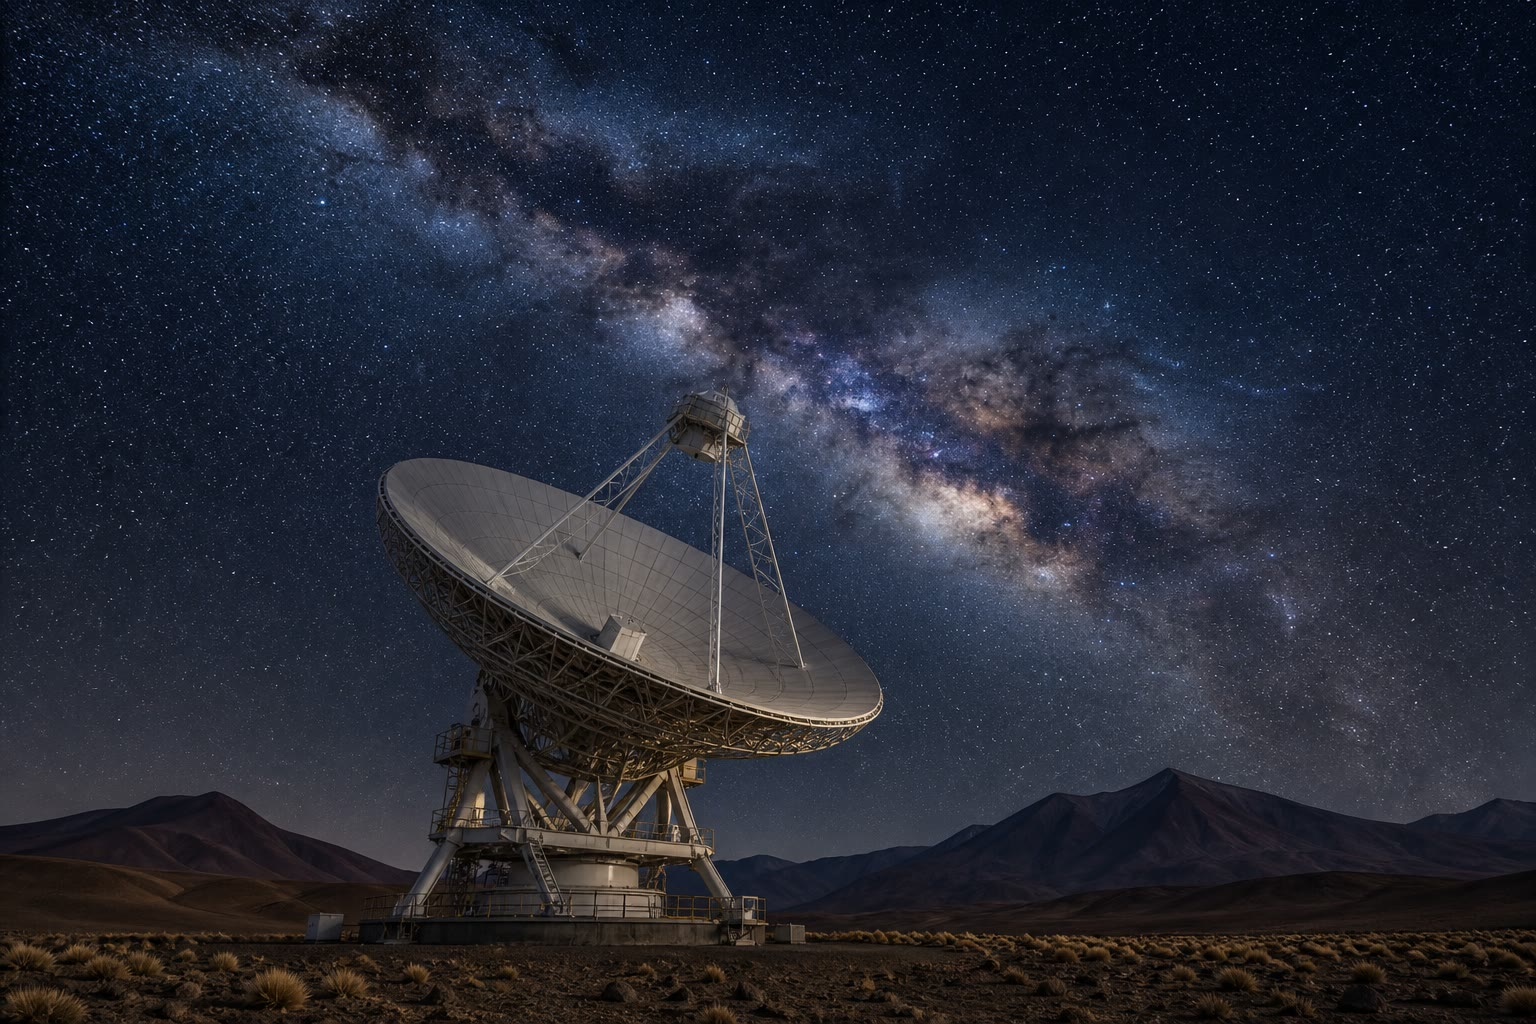
\includegraphics[width=0.58\linewidth]{images/book5/ai/b5-10-radio-dish.jpg}

{\small 银河之下的一座毫米波天线：它所聆听的星系悬于其上。射电天文学发现了宇宙微波背景 --- 那个 \qty{2.7}{K} 的嘶嘶声，原来是宇宙的起点。}
\end{omfigure}

\begin{omfigure}
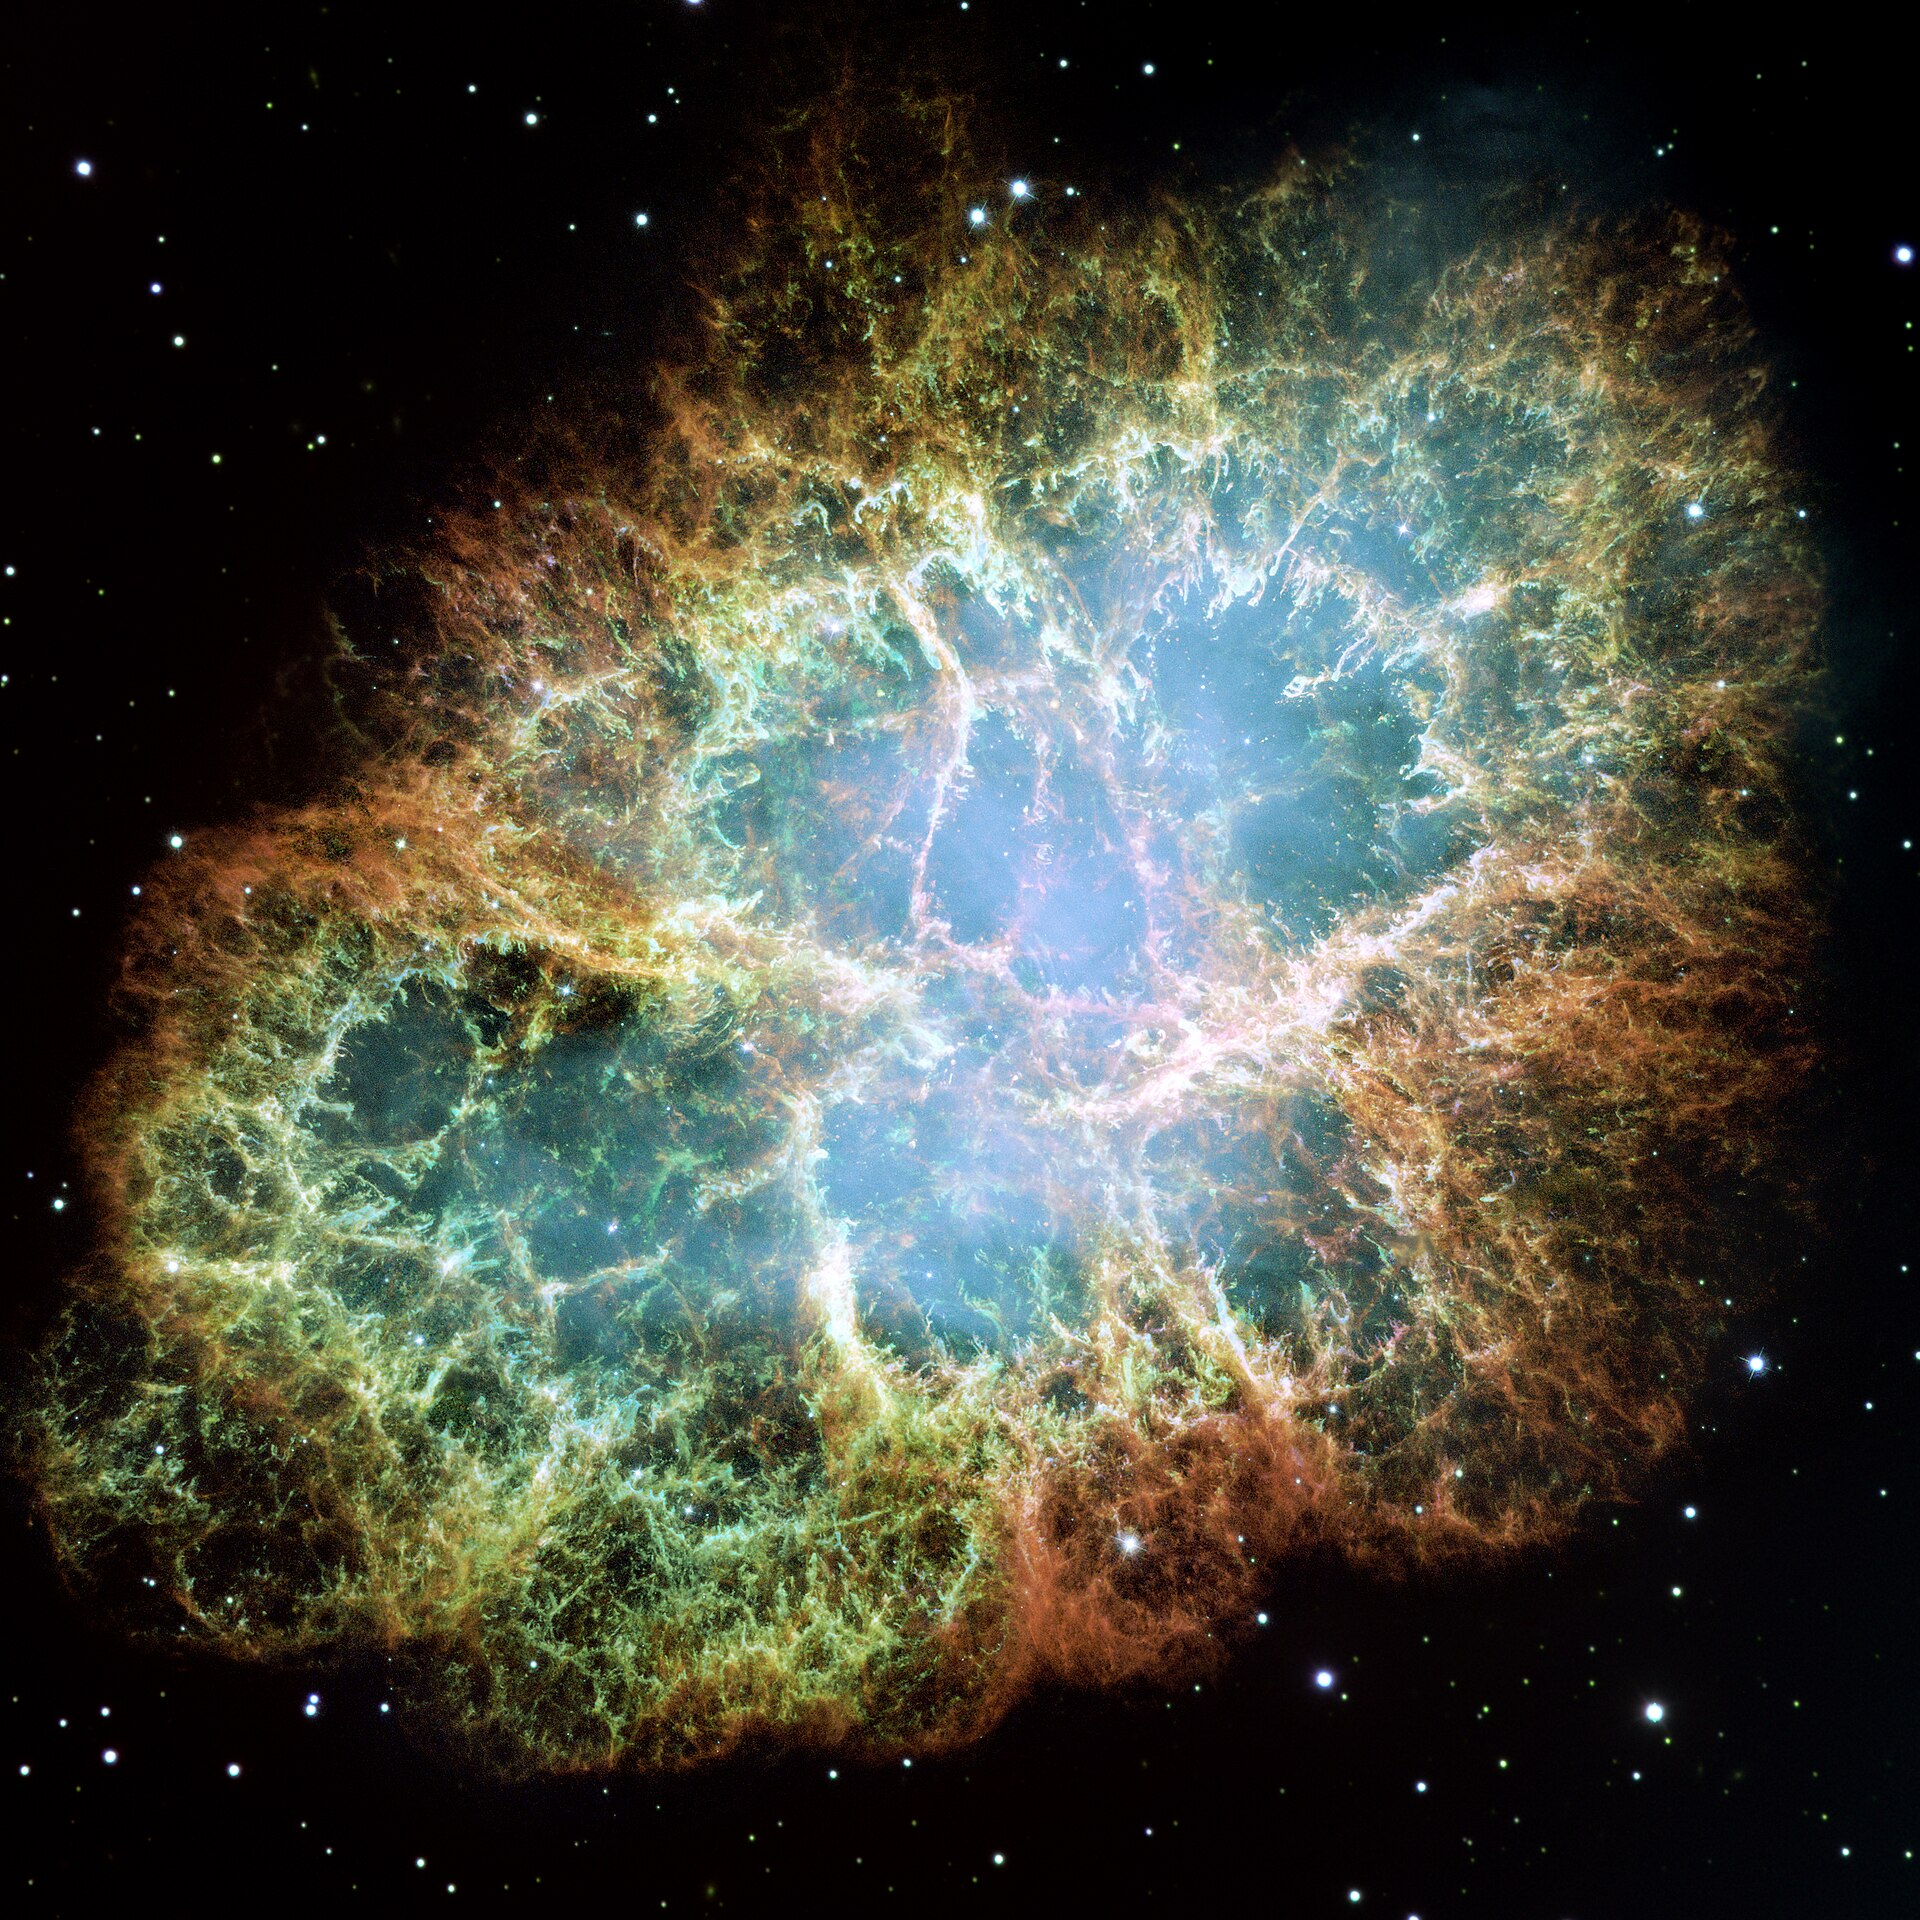
\includegraphics[width=0.6\linewidth]{images/book5/photo-crab-nebula.jpg}

{\small 蟹状星云（照片：NASA、ESA、J. Hester 与 A. Loll，公有领域）：公元 1054 年超新星的残骸，仍在膨胀，其核心是一颗中子星的毫秒脉冲“灯塔” --- 周末问题，九个世纪之后被拍摄下来。}
\end{omfigure}

\section{问题：恒星陨落的那一夜}

\begin{problem}\label{pb:b3:astrophysics:1}
\emph{恒星陨落的那一夜。}1987 年 2 月 23 日，一颗蓝
超巨星，位于大麦哲伦云中 --- $d \approx
\qty{50}{kpc} \approx \qty{1.5e21}{m}$ --- 成为 SN~1987A，这是
四个世纪以来最近的一次超新星。在任何望远镜看到它变亮的\emph{数小时前}，
三台地下探测器便已计数到
二十余个中微子。你要从第一性原理出发，
重建那一夜。

\medskip\noindent\textbf{第一部分 --- 曾经的恒星。}

\begin{enumerate}
  \item 该前身星质量约为 ${\sim}20\,M_\odot$。利用
        \cref{exo:b3:astrophysics:4}中的标度关系，估算其
        寿命，并与太阳的寿命相比较。
  \item 到其最后一天，恒星已成为洋葱状结构：H、He、C、O、Si
        壳层围绕铁核分布。为什么每一种接续的
        燃料都需要更热的核心？
  \item 为什么这一序列永久止于铁？
        （见\cref{prop:b3:nuclear-physics:binding}。）
  \item 惰性铁核向 $1.4\,M_\odot$ 增长。这个数字有何特殊之处，
        以及在那一质量下，
        哪一种压力失效了？
  \item 硅燃烧可维持恒星约
        \emph{一天}：这说明恒星的“时钟”
        在末期如何加速？
  \item 一旦压力支撑失效，对于密度
        为 $\sim\qty{e12}{kg/m^3}$ 的核心，自由落体
        大约需要多长时间（$t \sim 1/\sqrt{G\rho}$）？
\end{enumerate}

\medskip\noindent\textbf{第二部分 --- 中微子闪光。}

\begin{enumerate}[resume]
  \item 核心（$M \approx 1.4\,M_\odot = \qty{2.8e30}{kg}$）
        坍缩至 $R \approx \qty{12}{km}$：计算
        释放的引力能 $E \sim GM^2/R$。
  \item 与十亿个太阳持续发光
        一个月的光相比较（$L \sim 10^{9}L_\odot$，取 $\qty{2.6e6}{s}$）：
        说明光子只是一个舍入误差 --- 其余的
        99\,\% 去向何处，为什么只有中微子能
        迅速从坍缩的核心中逸出？
  \item 将 $E \approx \qty{3e46}{J}$ 分布于一个
        半径为 \qty{1.5e21}{m} 的球面上：计算
        到达地球时的能量注量。
  \item 每个中微子约 $\sim\qty{15}{MeV}$，计算
        数量注量（每 \unit{m^2} 的中微子数）。
  \item 一台探测器装有 \qty{2000}{t} 水：
        约含 ${\sim}1.5\times10^{32}$ 个自由质子。
        每个质子的相互作用概率为
        $\sigma \approx \qty{1e-46}{m^2}$（对每个反中微子，已给出），
        估算预期计数 --- 并与
        一台探测器记录的十一个相比较。
  \item 中微子比光早数小时到达。解释这两个
        “时钟”：是什么延迟了光子（变亮究竟
        发源于何处？），几乎同时的到达
        对中微子的质量说明了什么，
        对其速率又说明了什么？
  \item 二十五个被计数的中微子：各用一句话说明，
        它们证实了超新星理论的两件事。
\end{enumerate}

\medskip\noindent\textbf{第三部分 --- 剩下的是什么。}

\begin{enumerate}[resume]
  \item 计算半径为 \qty{12}{km}、
        质量为 $1.4\,M_\odot$ 的残余星的平均密度，并与
        \cref{def:b3:nuclear-physics:nuclide} 中的核
        密度作比较。
  \item 前身星核每 30 天自转一周，半径为
        $R \sim \qty{e5}{km}$：估计残余星的周期。
  \item 其磁场在磁通冻结下被放大
        $(R_0/R)^2$ 倍：由 \qty{e-2}{T} 出发，计算表面
        磁场。
  \item 解释“灯塔”模型：什么在扫过，什么在发出光束，
        以及为何蟹状星云脉冲星（诞生于 1054 年，被记载为白天出现的“客星”）
        至今仍每秒闪烁三十次。
  \item 若残余星质量超过 ${\sim}3\,M_\odot$：
        计算 $R_{\text{s}}$，取质量为 $3\,M_\odot$ 的情形，并说明其最终归宿。
  \item 脉冲星计时的稳定度达到 $10^{-15}$：
        举出一项利用如此精确、在天空中自转的“时钟”的物理应用。
\end{enumerate}

\medskip\noindent\textbf{第四部分 --- 它意味着什么。}

\begin{enumerate}[resume]
  \item 你呼吸的氧与血液中的铁：
        用两句话追溯每个原子的历程，从大爆炸产生的氢
        直至你的血液。
  \item Ia 型超新星（白矮星被推过
        $M_{\text{Ch}}$）时都在相同质量处爆炸，
        因而亮度几乎相同。解释为何这使它们成为
        \emph{标准烛光}，以及
        \cref{def:b3:astrophysics:hubble} 中的哈勃图
        是如何由它们构建的。
  \item 1998 年，遥远的 Ia 型超新星
        比哈勃直线所预言的要\emph{更暗}：
        陈述获得 2011 年诺贝尔奖的结论。
  \item 估计 SN~1987A 的光抵达时已传播了多少年
        --- 并说明它出发时地球上
        正在发生什么。
  \item 大麦哲伦云的中微子也穿过了你
        （当天所有活着的人）。每人大约有多少个穿过
        （${\sim}\qty{0.03}{m^2}$）？有人感觉到它吗
        （\cref{exo:b3:particle-physics:10}）？
  \item 用四句话结清本书的账目：一颗恒星
        靠隧道效应维持了一千万年的平衡；一次坍缩
        以中微子的形式付出代价；一具尸体由泡利
        不相容原理支撑；而残骸 --- 包括读者自己 ---
        仍随哈勃膨胀一同漂流。
\end{enumerate}
\end{problem}
